% Bản review tiếng Việt: cùng claim, hình, bảng và tài liệu tham khảo với bản tiếng Anh.
% Không áp dụng giới hạn sáu trang cho bản review.
\documentclass[conference]{IEEEtran}
\IEEEoverridecommandlockouts
\usepackage[T5]{fontenc}
\usepackage[utf8]{inputenc}
\usepackage[vietnamese]{babel}
\usepackage{times}
\usepackage{graphicx}
\graphicspath{{../../report/assets/}}
\usepackage{amsmath,amssymb}
\usepackage{booktabs}
\usepackage{array}
\usepackage{url}
\usepackage{balance}

\title{A Sensor-to-Brake AEB Pipeline in CARLA with Object-Level Radar, Camera Verification, and Limit-Finding Evaluation}

\author{
\IEEEauthorblockN{Mai Việt Hoàng và Phạm Đức An}
\IEEEauthorblockA{
\textit{Đại học Bách khoa Hà Nội}\\
Hà Nội, Việt Nam\\
hoangmai04222@gmail.com
}
}

\begin{document}
\maketitle

\begin{abstract}
Một mô phỏng phanh khẩn cấp tự động (AEB) có thể cho kết quả tốt nếu được cung
cấp trạng thái hoàn hảo của xe trước; bài toán khó hơn là tạo một mục tiêu ổn
định, có liên quan va chạm từ đầu ra cảm biến, rồi khép kín vòng điều khiển qua
chấp hành xe. Bài báo trình bày pipeline sensor-to-brake trong CARLA 0.9.11. Các
điểm radar phía trước được lọc theo hành lang quỹ đạo ego dự đoán, gom cụm và
theo dõi trước khi chọn mục tiêu. Radar giữ vai trò cung cấp khoảng cách, vận tốc
tương đối, thời gian tới va chạm (TTC) và biên khoảng cách dừng. YOLO26n tạo một
cổng cho phép ngữ nghĩa ở tầng muộn: lệnh phanh dự kiến chỉ được áp dụng nếu mục
tiêu radar đã chọn chiếu vào bounding box xe hiện tại hoặc vừa được camera xác
nhận. Luật staged PID chuyển rủi ro thành lệnh phanh CARLA. Đánh giá gồm 66 mô
phỏng đơn lượt với tick cố định: 24 case xe trước chạy chậm, 30 case xe trước
phanh và 12 case cut-in. Cả 38 case trong dải vận tốc mục tiêu đều đạt; 25/28
case stress đạt. Ba va chạm còn lại là CCRb tại 95 và 110~km/h với gap 20~m, và
cut-in muộn 100/60~km/h. Kết quả này ánh xạ một biên hoạt động theo cấu hình,
không ước lượng độ tin cậy an toàn. Công trình là baseline kỹ thuật minh bạch,
không tuyên bố một primitive fusion mới, chứng nhận NCAP hay kiểm định xe thật.
\end{abstract}

\begin{IEEEkeywords}
phanh khẩn cấp tự động, CARLA, xác nhận radar--camera, lựa chọn mục tiêu, TTC,
điều khiển xe
\end{IEEEkeywords}

\section{Giới thiệu}
AEB là bài toán vòng kín nhận thức--quyết định--chấp hành. Radar có thể đo khoảng
cách và vận tốc tương đối xuyên tâm, nhưng một điểm phản xạ chưa chắc đại diện
cho xe nằm trên đường đi của ego. Camera có thể nhận dạng xe nhưng không trực
tiếp cung cấp vận tốc đóng như radar. Hệ thống phanh phải giải quyết cả hai vấn
đề trước khi khoảng cách còn lại bị sử dụng hết. Vì vậy các tổng quan AEB xem
nhận thức môi trường, logic quyết định và thực thi điều khiển là một chuỗi phụ
thuộc lẫn nhau \cite{yang2022aebreview}.

Mô phỏng độ trung thực cao cho phép lặp lại các thí nghiệm gần va chạm trước khi
thử trên bãi \cite{dosovitskiy2017carla,kang2019testing}. Tuy nhiên mô phỏng cũng
tạo ra một bẫy phương pháp luận: simulator cung cấp actor ID, chuyển động chính
xác và bounding box ground truth. Nếu đưa các đại lượng này vào logic AEB online,
thí nghiệm chỉ kiểm tra controller với trạng thái mục tiêu lý tưởng thay vì hệ
sensor-to-brake. Do đó nghiên cứu này bắt đầu từ điểm radar CARLA và frame RGB.
Actor ID và động học actor không tham gia quyết định phanh, mặc dù hình học
simulator được dùng cho phép chiếu đã hiệu chuẩn và loại điểm mặt đường theo độ
cao. Ground truth chỉ dùng tạo nhãn offline và chấm kết quả.

Không thành phần riêng lẻ nào--ghép hình học, TTC, khoảng cách dừng, liên quan
quỹ đạo hay phanh phân tầng--được tuyên bố là mới. Đóng góp nằm ở một cấu hình có
thể truy vết của các khối này và cách đánh giá giữ nguyên các case fail. Cụ thể:
1) tầng point-to-object cho radar CARLA với lọc quỹ đạo, gom cụm tất định và xác
nhận theo thời gian; 2) chuỗi rủi ro do radar cung cấp kết hợp cổng cho phép ngữ
nghĩa YOLO ở tầng muộn, không sử dụng actor ID hoặc trạng thái xe ground truth
trong quyết định online; 3) chấp hành staged PID vòng kín với log tick cố định;
và 4) đánh giá tham số hóa tách dải vận tốc mục tiêu với case tìm giới hạn, đồng
thời báo cáo đủ ba va chạm.

\section{Công trình liên quan và định vị}
AEB radar--camera đã xuất hiện trước nghiên cứu này. Kim và Song ghép radar và
thị giác để nhận dạng xe \cite{kim2013vehicle}; Hsu \emph{và cs.} xử lý nhiễu
radar/camera khi chọn mục tiêu AEB \cite{hsu2015noise}. Liên kết hình học với xe
nằm trong quỹ đạo cũng đã được chứng minh bằng LiDAR và camera trên xe thật
\cite{bae2021cipv}. Về quyết định và điều khiển, Zhang \emph{và cs.} kết hợp nhận
dạng mục tiêu trên đường cong, TTC, khoảng cách an toàn và phanh phân tầng trong
CarSim/Simulink \cite{zhang2023curved}. Vì vậy lọc theo quỹ đạo và phanh nhiều
tiêu chí không phải đóng góp đầu tiên của bài báo này.

CARLA cũng đã được dùng để validation pipeline tự lái đầy đủ bằng các kịch bản
xây dựng từ protocol \cite{gomez2022carla}. Riêng với AEB, Feng \emph{và cs.}
đánh giá nhận thức bằng event camera trong CARLA \cite{feng2025dvs}. Akula
\emph{và cs.} xây dựng bộ xác nhận camera do radar dẫn hướng trên xe thử nghiệm,
thay nhận dạng toàn ảnh bằng mật độ cạnh trong vùng radar
\cite{akula2026radarguided}. Vai trò camera trong nghiên cứu hiện tại có cùng
tư tưởng nhưng dùng YOLO để xác nhận ngữ nghĩa lớp \emph{car}. Trọng tâm khác
biệt là chuyển điểm radar CARLA thành track, rủi ro động học có xét quỹ đạo,
chấp hành staged PID và sweep biên car-to-car gồm 66 case. Bảng~\ref{tab:positioning}
tóm tắt định vị này. Bảng hỗ trợ claim tích hợp hệ thống, không hỗ trợ claim
thuật toán đầu tiên.

\begin{table*}[t]
\caption{Định vị với một số nghiên cứu AEB và fusion mục tiêu trong quỹ đạo.}
\label{tab:positioning}
\centering
\footnotesize
\begin{tabular}{p{0.15\textwidth}p{0.25\textwidth}p{0.25\textwidth}p{0.25\textwidth}}
\toprule
Nghiên cứu & Nhận thức / vai trò mục tiêu & Quyết định hoặc chấp hành & Trọng tâm đánh giá \\
\midrule
Kim và Song \cite{kim2013vehicle} & Nhận dạng xe bằng radar--vision & Nhận dạng mục tiêu hướng AEB & Nhận dạng bằng sensor fusion \\
Bae \emph{và cs.} \cite{bae2021cipv} & Chiếu LiDAR và camera tracking để tìm xe gần nhất trong quỹ đạo & Ứng dụng AEB lấy cảm hứng Euro NCAP & Kịch bản xe thật \\
Zhang \emph{và cs.} \cite{zhang2023curved} & Chọn mục tiêu nguy hiểm trên đường cong & Kết hợp TTC/khoảng cách an toàn và phanh phân tầng & CarSim/Simulink \\
Feng \emph{và cs.} \cite{feng2025dvs} & So sánh detection event camera và RGB & Nhận dạng hình ảnh sớm hơn cho AEB & Kịch bản DVS trong CARLA \\
Akula \emph{và cs.} \cite{akula2026radarguided} & Track radar ô tô và xác nhận camera bằng mật độ cạnh & TTC và brake-by-wire & 72 phiên chạy thật; 33 threat có dàn dựng \\
Nghiên cứu này & Điểm radar CARLA thành track; path gate; cổng YOLO & TTC, biên dừng, staged PID, chấp hành CARLA & 66 case fixed-tick CCRm, CCRb và cut-in \\
\bottomrule
\end{tabular}
\end{table*}

\section{Pipeline sensor-to-brake được đánh giá}
\subsection{Phạm vi và ranh giới thông tin}
Hệ thống dùng Tesla Model 3 trong Town04 với thời tiết lý tưởng. Camera RGB sau
kính lái và radar cản trước chạy ở 20~Hz. Radar CARLA là cảm biến detection trừu
tượng, không phải chuỗi tín hiệu FMCW raw; độ trung thực radar ảo thay đổi mạnh
theo cấp mô hình \cite{magosi2022radar}. Vì vậy bài báo chỉ claim validation
logic, không claim validation xử lý tín hiệu radar.

Hình~\ref{fig:pipeline} thể hiện ranh giới thông tin online. Transform cảm biến
chính xác dùng hiệu chuẩn phép chiếu radar--ảnh; truy vấn waypoint bản đồ CARLA
ước lượng độ cao mặt đường để loại ground. Đây là hình học đặc quyền của
simulator và được công bố rõ. Khi phanh, hệ thống không truy vấn actor ID, vận
tốc actor, nhãn làn actor hay bounding box 2-D/3-D ground truth. Các thông tin đó
chỉ dùng offline để tạo nhãn YOLO và chấm collision, gap, target role.

\begin{figure*}[t]
  \centering
  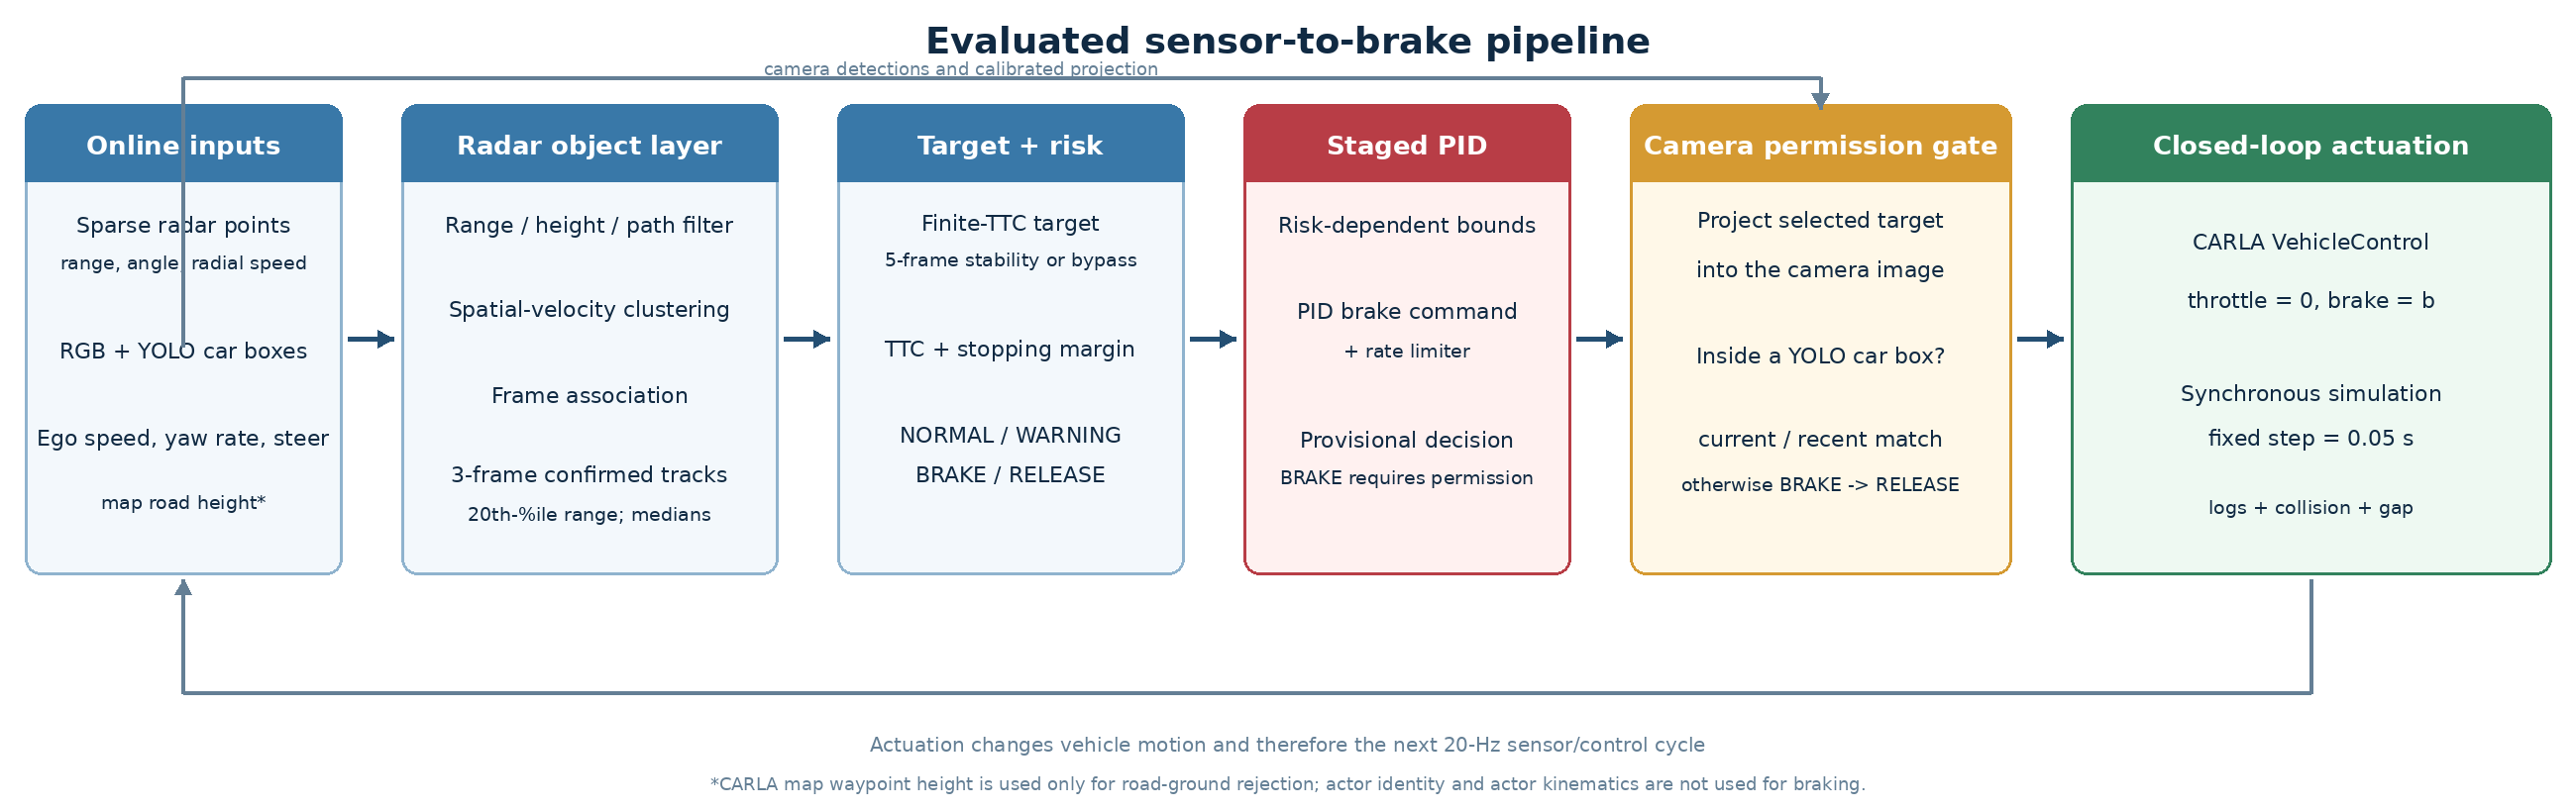
\includegraphics[width=0.98\textwidth]{aeb_closed_loop_architecture_en.png}
  \caption{Vòng kín được đánh giá. Radar tạo mục tiêu động học và quyết định AEB
  dự kiến; liên kết camera là cổng cho phép đối với \texttt{BRAKE}. Dấu sao chỉ
  truy vấn map-height đã công bố.}
  \label{fig:pipeline}
\end{figure*}

\subsection{Thứ tự thực thi online}
Thứ tự các khối quan trọng vì camera không được phép tự tạo rủi ro động học. Ở
mỗi lần radar cập nhật, hệ thống: (1) lấy trạng thái ego và cập nhật quỹ đạo độ
cong không đổi; (2) loại điểm radar ngoài gate range, độ cao, ground và quỹ đạo;
(3) gom cụm và ghép với track đang có; (4) tạo danh sách
\texttt{RadarObject} và chọn một target đã xác nhận; (5) tính TTC, khoảng cách
dừng yêu cầu, trạng thái giám sát và lệnh phanh dự kiến; (6) chạy YOLO trên frame
RGB mới nhất và chiếu target radar đã chọn lên ảnh; (7) chỉ cho phép
\texttt{BRAKE} nếu liên kết ảnh đang có hoặc được giữ ngắn hạn; và (8) áp dụng
\texttt{VehicleControl}, sau đó log trạng thái xe ở tick đồng bộ tiếp theo.

Thứ tự này quy định rõ quyền sở hữu thông tin. Một box YOLO không có target radar
không thể phanh vì thiếu vận tốc tương đối và khoảng cách của công thức rủi ro.
Ngược lại, object radar đang tiến gần có thể tạo \texttt{WARNING}, nhưng
\texttt{BRAKE} dự kiến bị chặn nếu thiếu liên kết ảnh gần đây. Thiết kế bảo thủ
với radar false positive nhưng dễ bị ảnh hưởng bởi camera miss; tính bất đối
xứng này được phân tích ở kết quả cut-in. Inference đặt mỗi 0.15~s, chậm hơn tick
cảm biến 0.05~s, nên cửa sổ giữ xác nhận ngắn là một phần hành vi đánh giá chứ
không chỉ phục vụ hiển thị.

\subsection{Radar object, liên quan quỹ đạo và chọn mục tiêu}
Quỹ đạo độ cong không đổi được ước lượng từ tốc độ ego, yaw rate và góc lái. Với
độ cong $\kappa$ và chiều dài cung $s$,
\begin{equation}
 x(s)=\frac{\sin(\kappa s)}{\kappa},\qquad
 y(s)=\frac{1-\cos(\kappa s)}{\kappa},
 \label{eq:path}
\end{equation}
và chuyển sang giới hạn đường thẳng khi $\kappa\approx0$. Horizon bị giới hạn
bởi radar 100~m và look-ahead 2.5~s theo tốc độ. Điểm ngoài gate range, độ cao,
ground hoặc cách quỹ đạo quá 1.25~m bị loại.

Các điểm còn lại được nối nếu khoảng cách phẳng, khoảng cách đứng và chênh vận
tốc xuyên tâm không vượt 1.0~m, 1.5~m và 2.0~m/s. Tọa độ dọc cụm lấy percentile
20; tọa độ ngang, độ cao và vận tốc tương đối lấy median. Ghép greedy so sánh vị
trí dự đoán và vận tốc giữa các frame. Track cần ba hit liên tiếp và trở thành
stale ngay khi miss. Track confirmed, không stale được xếp theo TTC hữu hạn rồi
đến range. Target đã chọn phải tồn tại năm frame, trừ khi khoảng cách dọc không
quá 22~m hoặc biên dừng không quá $-4$~m để bật risk bypass. Track không match
bị xóa sau bốn update miss. Đây là quy tắc kỹ thuật tất định, không phải Kalman,
tracker xác suất hay xác suất tồn tại đã hiệu chuẩn.

Hai gate thời gian có mục đích khác nhau. Ba hit radar chứng minh cụm tồn tại;
năm lần chọn target cho thấy cùng track tiếp tục là ứng viên rủi ro nhất. Risk
bypass giúp tránh mọi độ trễ là bắt buộc. Ở 20~Hz, một cụm sạch được xác nhận ở
mẫu thứ ba (0.10~s sau mẫu đầu); vì đếm target bắt đầu tại đó, target đạt năm lần
chọn ở mẫu thứ bảy (0.30~s sau mẫu đầu) nếu không bypass. Association và thời
điểm sensor có thể thay đổi tick sử dụng đầu tiên.

\subsection{Xác nhận camera}
YOLO26n \cite{ultralytics_yolo} được fine-tune cho một lớp \emph{car} bằng nhãn
CARLA. Chỉ khi thu dữ liệu, bounding box 3-D actor nhìn thấy được chiếu lên ảnh
runtime và đổi sang nhãn YOLO. Session được tách giữa train, validation và test;
16--21\% ảnh empty được giữ để tạo negative frame. AEB online không nhận các
nhãn này.

Ba split có 1,505/300/200 ảnh và 1,872/379/264 box. Training dùng ảnh
$640\!\times\!640$, 100 epoch, batch 16, AdamW, learning rate đầu 0.001 và seed
2026. Ở epoch tốt nhất được báo cáo, precision, recall, $\mathrm{mAP}_{50}$ và
$\mathrm{mAP}_{50:95}$ là 0.9919, 0.9642, 0.9940 và 0.9495. Hình~\ref{fig:yolo}
cho thấy lịch sử training được check-in. Các giá trị này chỉ chứng minh khả năng
phù hợp hẹp trong domain; chúng không đo accuracy liên kết end-to-end hoặc khả
năng chuyển sang ngoài Town04 và điều kiện ảnh thuận lợi.

\begin{figure}[t]
  \centering
  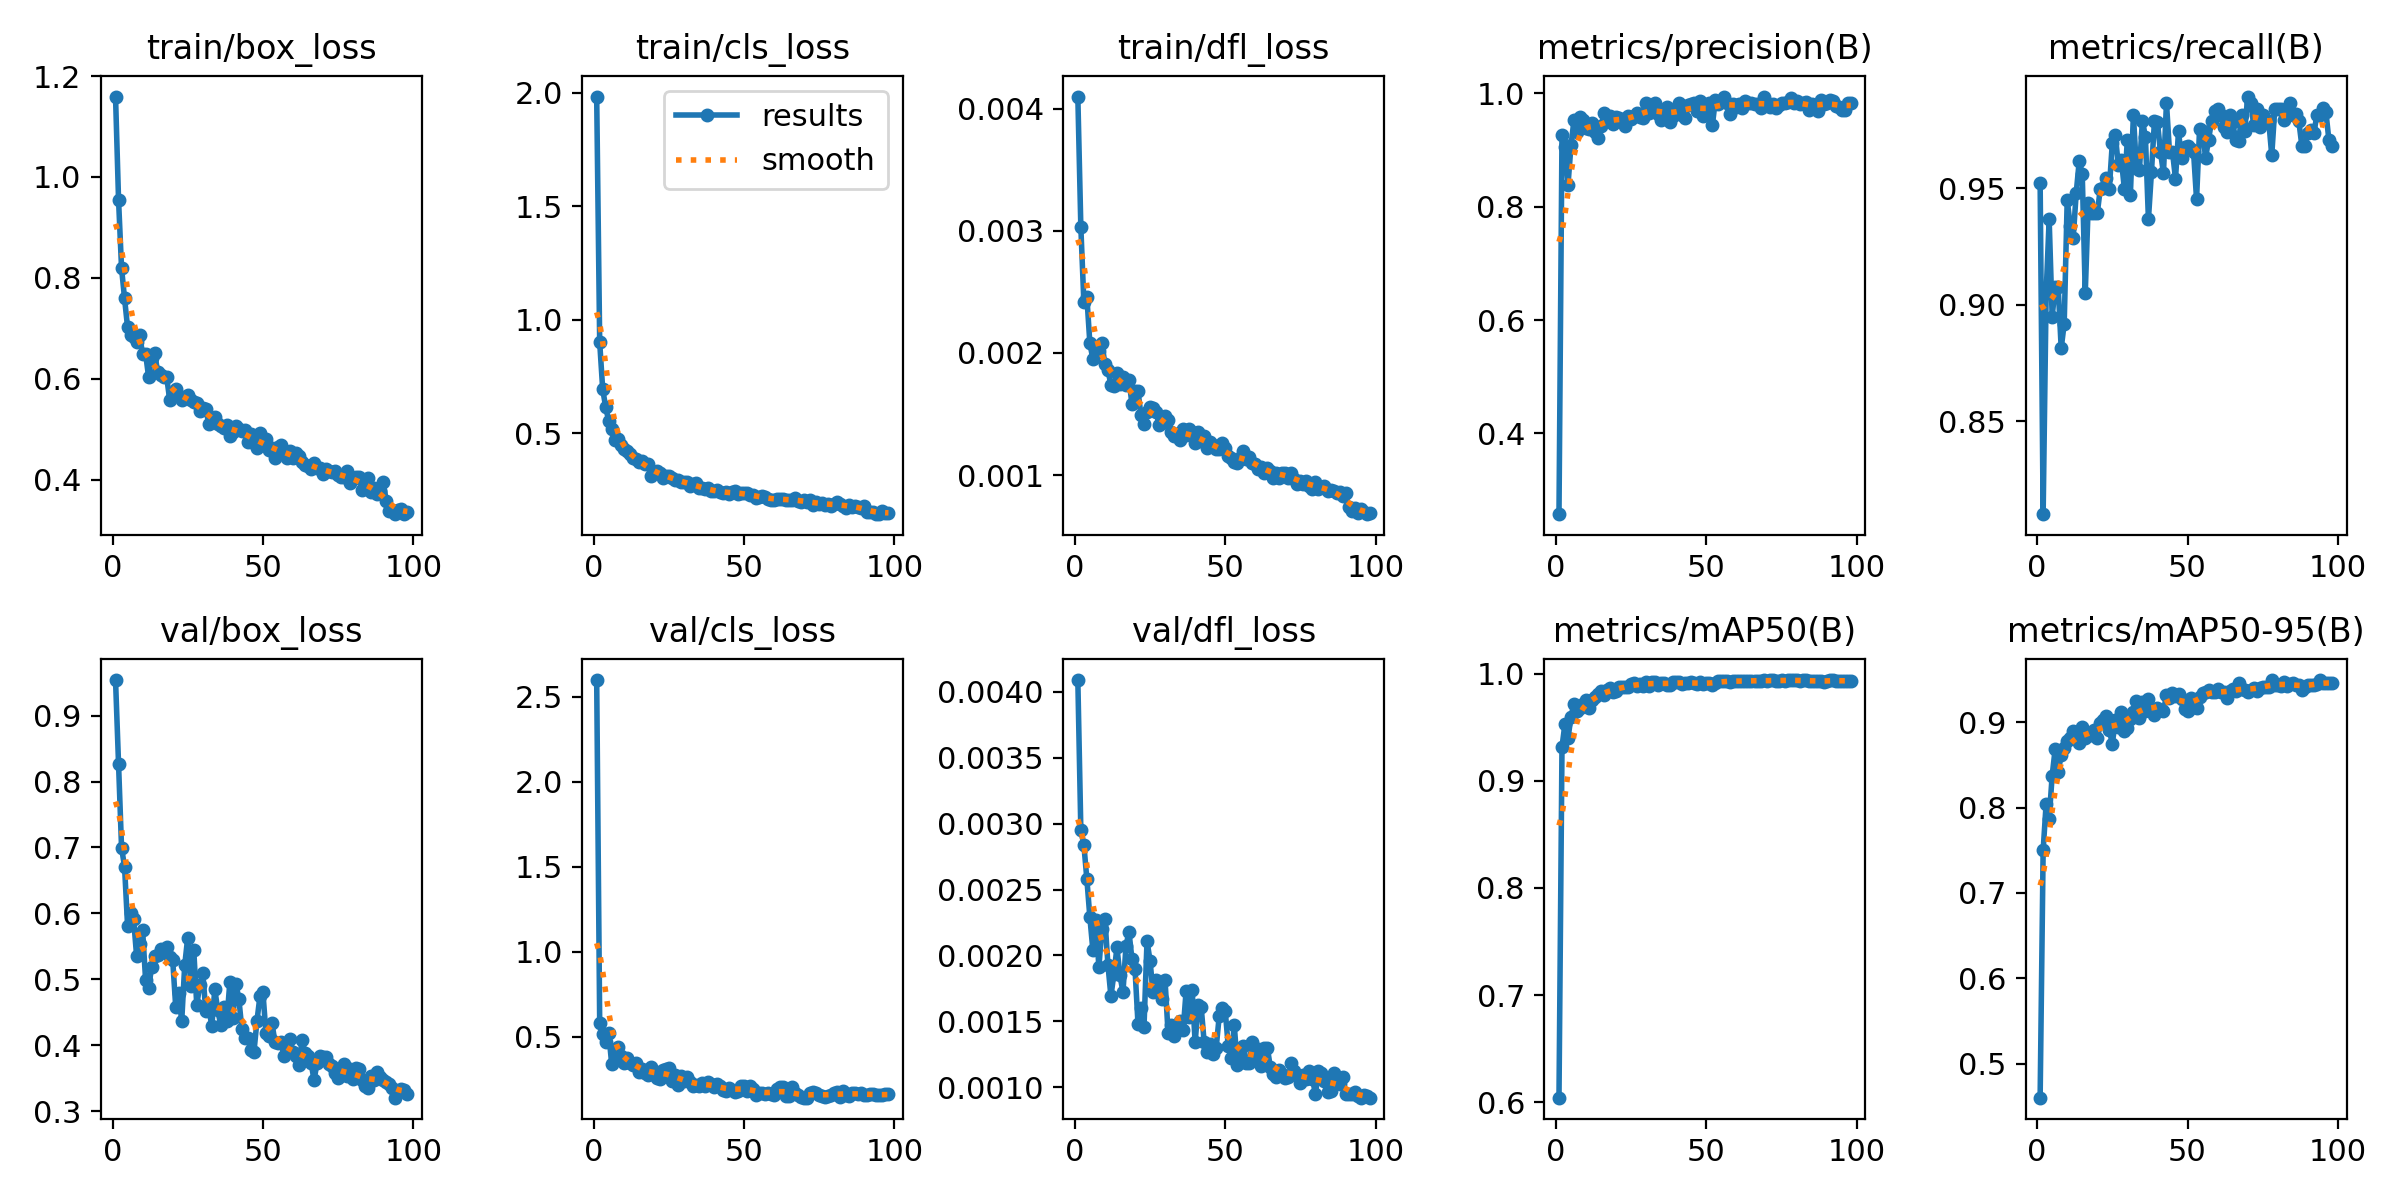
\includegraphics[width=0.96\columnwidth]{evidence/yolo_training_results.png}
  \caption{Lịch sử train/validation của YOLO26n một lớp dùng để xác nhận. Chỉ số
  detector không được coi là chỉ số an toàn AEB.}
  \label{fig:yolo}
\end{figure}

Với target trong hệ camera $(X_c,Y_c,Z_c)$,
\begin{equation}
 u=f_xX_c/Z_c+c_x,\qquad v=f_yY_c/Z_c+c_y,\quad Z_c>0.
 \label{eq:projection}
\end{equation}
Liên kết hợp lệ nếu $(u,v)$ nằm trong box YOLO lớp xe sau NMS. Chỉ
\texttt{BRAKE} dự kiến bị gate: match hiện tại hoặc vừa được giữ sẽ cho đi qua;
nếu không, lệnh thành \texttt{RELEASE} với brake bằng 0. Bản được đánh giá giữ
xác nhận 0.35~s theo monotonic clock của host. Radar vẫn là nguồn duy nhất của
khoảng cách và vận tốc tương đối. Đây là decision gating muộn, không phải fusion
đa đối tượng chung.

\subsection{Rủi ro và chấp hành staged PID}
Với khoảng cách dọc $d$ và vận tốc tương đối radar $v_r$ (âm khi tiến gần),
\begin{equation}
 v_c=-v_r,\qquad \mathrm{TTC}=d/v_c\quad(v_c>0).
 \label{eq:ttc}
\end{equation}
Với tốc độ ego $v_e$ và $v_t=\max(0,v_e+v_r)$, khoảng cách yêu cầu là
\begin{equation}
 d_{\rm req}=\max\!\left(d_0, v_et_r+\frac{v_e^2}{2a_e}
 -\frac{v_t^2}{2a_t}+d_0\right),\quad m=d-d_{\rm req}.
 \label{eq:stopping}
\end{equation}
Trong đó $t_r=0.20$~s, $a_e=8.0$~m/s$^2$, $a_t=6.0$~m/s$^2$, $d_0=1.0$~m là
tham số mô hình rủi ro, không phải đại lượng đo trên phần cứng.

Các trạng thái giám sát là \texttt{NORMAL}, \texttt{WARNING}, \texttt{BRAKE} và
\texttt{RELEASE}. Trong \texttt{BRAKE}, sai số PID kết hợp thiếu hụt margin và
TTC:
\begin{equation}
\begin{aligned}
 e&=\max(0,m_{\rm th}-m-\delta_m)+k_t\max(0,T_b-\mathrm{TTC}),\\
 b&=\operatorname{clip}\!\left(b_0+K_pe+K_i\!\int e\,dt+K_d\dot e\right).
\end{aligned}
\label{eq:pid}
\end{equation}
Đầu ra được rate-limit và clip theo bound soft, medium, hard hoặc emergency
(0.55, 0.75, 0.90 và 1.00). Khoảng cách không quá 18~m, margin không quá $-5$~m
hoặc TTC không quá 0.80~s mở tầng emergency. Hard khả dụng nếu TTC không quá
1.10~s hoặc margin không quá $-2$~m. Integral bị chặn, chỉ giữ đạo hàm sai số
dương, tốc độ tăng/giảm lệnh bị giới hạn. Logic trạng thái có hold tối thiểu
0.3~s và release TTC 3.5~s. Trong batch đánh giá,
\texttt{hold\_brake\_until\_stopped} được bật, nên controller dự kiến giữ
\texttt{BRAKE} qua pha dừng trừ khi camera permission chặn; trạng thái điều khiển
được reset giữa các scenario.

Vì vậy nhãn tầng là schedule lệnh bên trong \texttt{BRAKE}, không phải trạng thái
giám sát độc lập. Thiết kế cũng không phải controller tối ưu comfort: $K_d=0$
trong cấu hình cuối và mục tiêu không có ràng buộc gia tốc/jerk. Staging làm rõ
bound theo rủi ro trong khi giữ lệnh liên tục. Bảng~\ref{tab:config} liệt kê tham
số chính.

\begin{table}[t]
\caption{Cấu hình đánh giá chính.}
\label{tab:config}
\centering
\footnotesize
\begin{tabular}{p{0.56\columnwidth}p{0.31\columnwidth}}
\toprule
Thành phần & Giá trị \\
\midrule
Camera / FOV / tick & 1280$\times$720 / 70$^\circ$ / 0.05 s \\
Radar range / FOV / rate & 100 m / 30$^\circ$$\times$6$^\circ$ / 2000 điểm/s \\
Xác nhận track / target chọn & 3 / 5 frame \\
TTC warning / brake / release & 3.0 / 1.5 / 3.5 s \\
PID $K_p,K_i,K_d,k_t$ & 0.12, 0.01, 0, 0.12 \\
Tốc độ tăng brake / emergency & 3.0 / 20.0 s$^{-1}$ \\
TTC hard / emergency & 1.10 / 0.80 s \\
Margin hard / emergency & $-2.0$ / $-5.0$ m \\
\bottomrule
\end{tabular}
\end{table}

\section{Thiết kế thực nghiệm}
Simulator chạy đồng bộ với bước 0.05~s và điều khiển throttle/brake theo physics.
Tập cuối chỉ gồm case nguy hiểm; mọi case đều kỳ vọng có phanh và không va chạm.
PASS yêu cầu đồng thời: (1) có brake override, (2) CARLA không báo collision,
(3) minimum bumper gap ít nhất 0.5~m và (4) độ lệch tâm làn lớn nhất không quá
1.25~m. Clear-road, adjacent-lane, curve, cut-out và multi-actor là kiểm tra
trong quá trình phát triển nhưng không nằm trong aggregate 66 case, nên không
thể dùng để claim định lượng về false brake.

Mọi case dùng cùng vùng spawn Town04 và physics speed controller. CCRm giữ xe
trước chậm hơn ego 30~km/h. CCRb bắt đầu với ego và lead cùng tốc độ; lead phanh
1.0 tại 1.5~s. Cut-in spawn hazard ở làn trái, bắt đầu đổi sang phải tại 1.0~s và
yêu cầu actor gây phanh phải là xe cut-in. Ba họ lần lượt tách vận tốc đóng ổn
định, thay đổi gia tốc lead và thay đổi liên quan quỹ đạo ngang. Chúng không tái
tạo đầy đủ apparatus hoặc tolerance Euro NCAP.

Mỗi tick ghi simulator time, tốc độ/gia tốc ego, lane offset, collision count,
khoảng cách center và bumper tới hazard cấu hình, số candidate/cluster radar,
track được chọn, TTC, khoảng cách yêu cầu, margin, trạng thái AEB và lệnh phanh.
Ghép actor ground truth chỉ nằm trong logger để kiểm tra target đã chọn có đúng
hazard. Timing định lượng dùng simulation tick thay vì FPS video; UI/video chỉ
là diagnostic.

\subsection{Ngữ nghĩa đo lường và truy vết}
Hai loại khoảng cách không được trộn lẫn. Controller AEB dùng tọa độ dọc của
radar object đã chọn. Ngược lại, \emph{bumper gap} trong báo cáo là đại lượng
đánh giá: runner chiếu tâm hazard lên trục tiến ego rồi trừ nửa chiều dài bounding
box hai actor. ``Brake gap'' là gap đánh giá tại tick đầu tiên có AEB override;
``minimum gap'' là giá trị nhỏ nhất toàn run. Collision event CARLA là tín hiệu
chấm độc lập. Vì vậy ground truth dùng để đánh giá một quyết định từ cảm biến,
không dùng để tạo quyết định.

Cấu hình nằm ở \path{configs/sensors.yaml}; 66 case nằm tại
\path{configs/scenarios/suites/system_limit_extended_sweep.yaml}.
\path{radar_object_tracker.py}, \path{radar_aeb_pipeline.py},
\path{brake.py} và \path{run_fusion_aeb_scenarios.py} cài đặt bốn tầng chính.
Script tạo CSV từng tick, summary từng case và aggregate JSON. Mapping module/cấu
hình được nêu vì bảng tham số không đủ mô tả thứ tự chạy, bypass hoặc stale track.

ODD được giới hạn là cao tốc Town04, chỉ xe ô tô, thời tiết lý tưởng và các cảm
biến mô phỏng đã nêu. Trong ODD này, Bảng~\ref{tab:suite} chia tổ hợp vận tốc
thành \emph{dải mục tiêu} và \emph{dải stress}; bản thân hai subset không phải
hai ODD. Mỗi tổ hợp sweep các gap. Mỗi cấu hình chỉ chạy một lần nên kết quả đo
coverage case cấu hình, không phải xác suất vận hành an toàn.

\begin{table}[t]
\caption{Tập cuối 66 case. Mỗi bộ vận tốc được kết hợp với toàn bộ gap liệt kê.}
\label{tab:suite}
\centering
\scriptsize
\begin{tabular}{p{0.17\columnwidth}p{0.37\columnwidth}p{0.27\columnwidth}}
\toprule
Họ & Dải mục tiêu & Dải stress \\
\midrule
CCRm & ego/lead 60/30, 80/50; gap 20,30,40,50,60,80 m (12) & 100/70, 110/80; cùng gap (12) \\
CCRb & ego 50,65,80; gap 20,30,40,50,60,80 m (18) & ego 95,110; cùng gap (12) \\
Cut-in & ego/lead 60/40, 80/50; gap 25,35,45,60 m (8) & 100/60; cùng gap (4) \\
\midrule
Tổng & 38 case & 28 case \\
\bottomrule
\end{tabular}
\end{table}

\section{Kết quả và thảo luận}
\subsection{Kết quả theo case cấu hình}
Bảng~\ref{tab:results} cho kết quả 38/38 dải mục tiêu và 25/28 stress. CCRm đạt
24/24 vì vận tốc đóng 30~km/h vẫn vừa phải dù tốc độ ego tuyệt đối cao. Các fail
chỉ xuất hiện ở CCRb 95 và 110~km/h với gap 20~m, và cut-in 100/60~km/h gap
25~m.

\begin{table}[t]
\caption{Kết quả theo họ và subset đánh giá.}
\label{tab:results}
\centering
\footnotesize
\begin{tabular}{lrrr|rrr}
\toprule
& \multicolumn{3}{c|}{Mục tiêu} & \multicolumn{3}{c}{Stress} \\
Họ & N & P & F & N & P & F \\
\midrule
CCRm & 12 & 12 & 0 & 12 & 12 & 0 \\
CCRb & 18 & 18 & 0 & 12 & 10 & 2 \\
Cut-in & 8 & 8 & 0 & 4 & 3 & 1 \\
\midrule
Tổng & 38 & 38 & 0 & 28 & 25 & 3 \\
\bottomrule
\end{tabular}
\end{table}

Grid CCRb trong Bảng~\ref{tab:ccrbmap} cho thấy giới hạn cục bộ thay vì mọi case
tốc độ cao đều fail. Cả hai collision chỉ ở cột 20~m; mọi gap 30--80~m đều đạt.
Tương tự, cut-in 100/60~km/h fail ở 25~m nhưng đạt tại 35, 45, 60~m. Evidence mô
tả tương tác tốc độ--gap--maneuver, không phải ngưỡng tốc độ phổ quát.

\begin{table}[t]
\caption{Bản đồ CCRb (P: đạt; C: collision).}
\label{tab:ccrbmap}
\centering
\scriptsize
\begin{tabular}{c*{6}{c}}
\toprule
Tốc độ ego & 20 m & 30 m & 40 m & 50 m & 60 m & 80 m \\
\midrule
50 km/h  & P & P & P & P & P & P \\
65 km/h  & P & P & P & P & P & P \\
80 km/h  & P & P & P & P & P & P \\
95 km/h  & C & P & P & P & P & P \\
110 km/h & C & P & P & P & P & P \\
\bottomrule
\end{tabular}
\end{table}

Log đại diện trong Bảng~\ref{tab:boundary} phân biệt tốc độ tuyệt đối với động
học đóng. CCRm 110/80 bắt đầu phanh ở 18.96~m nhưng giữ 15.01~m, trong khi lead
phanh làm mất chuyển động thuận lợi đó. Cùng gap đầu 20~m, CCRb đạt ở 80~km/h với
1.96~m còn lại nhưng collision tại 95 và 110~km/h. Case fail 95~km/h vẫn có lệnh
phanh (Hình~\ref{fig:ccrb}); do đó evidence hỗ trợ biên thiếu khoảng cách của cả
chuỗi cấu hình, không chứng minh perception bỏ lỡ lead.

\begin{table}[t]
\caption{Case biên đại diện từ report và evidence summary được check-in.}
\label{tab:boundary}
\centering
\scriptsize
\setlength{\tabcolsep}{3pt}
\begin{tabular}{p{0.43\columnwidth}rrl}
\toprule
Scenario & Brake gap (m) & Min. gap (m) & Kết quả \\
\midrule
ccrm\_110\_80\_gap\_20 & 18.96 & 15.01 & Đạt \\
ccrb\_80\_gap\_20 & 18.56 & 1.96 & Đạt \\
ccrb\_95\_gap\_20 & 18.56 & 0.0134 & Collision \\
ccrb\_110\_gap\_20 & -- & 0.0806 & Collision \\
cutin\_80\_50\_gap\_25 & 10.46 & 5.51 & Đạt \\
cutin\_100\_60\_gap\_25 & 7.26 & 0.4763 & Collision \\
\bottomrule
\end{tabular}
\end{table}

\begin{figure}[t]
  \centering
  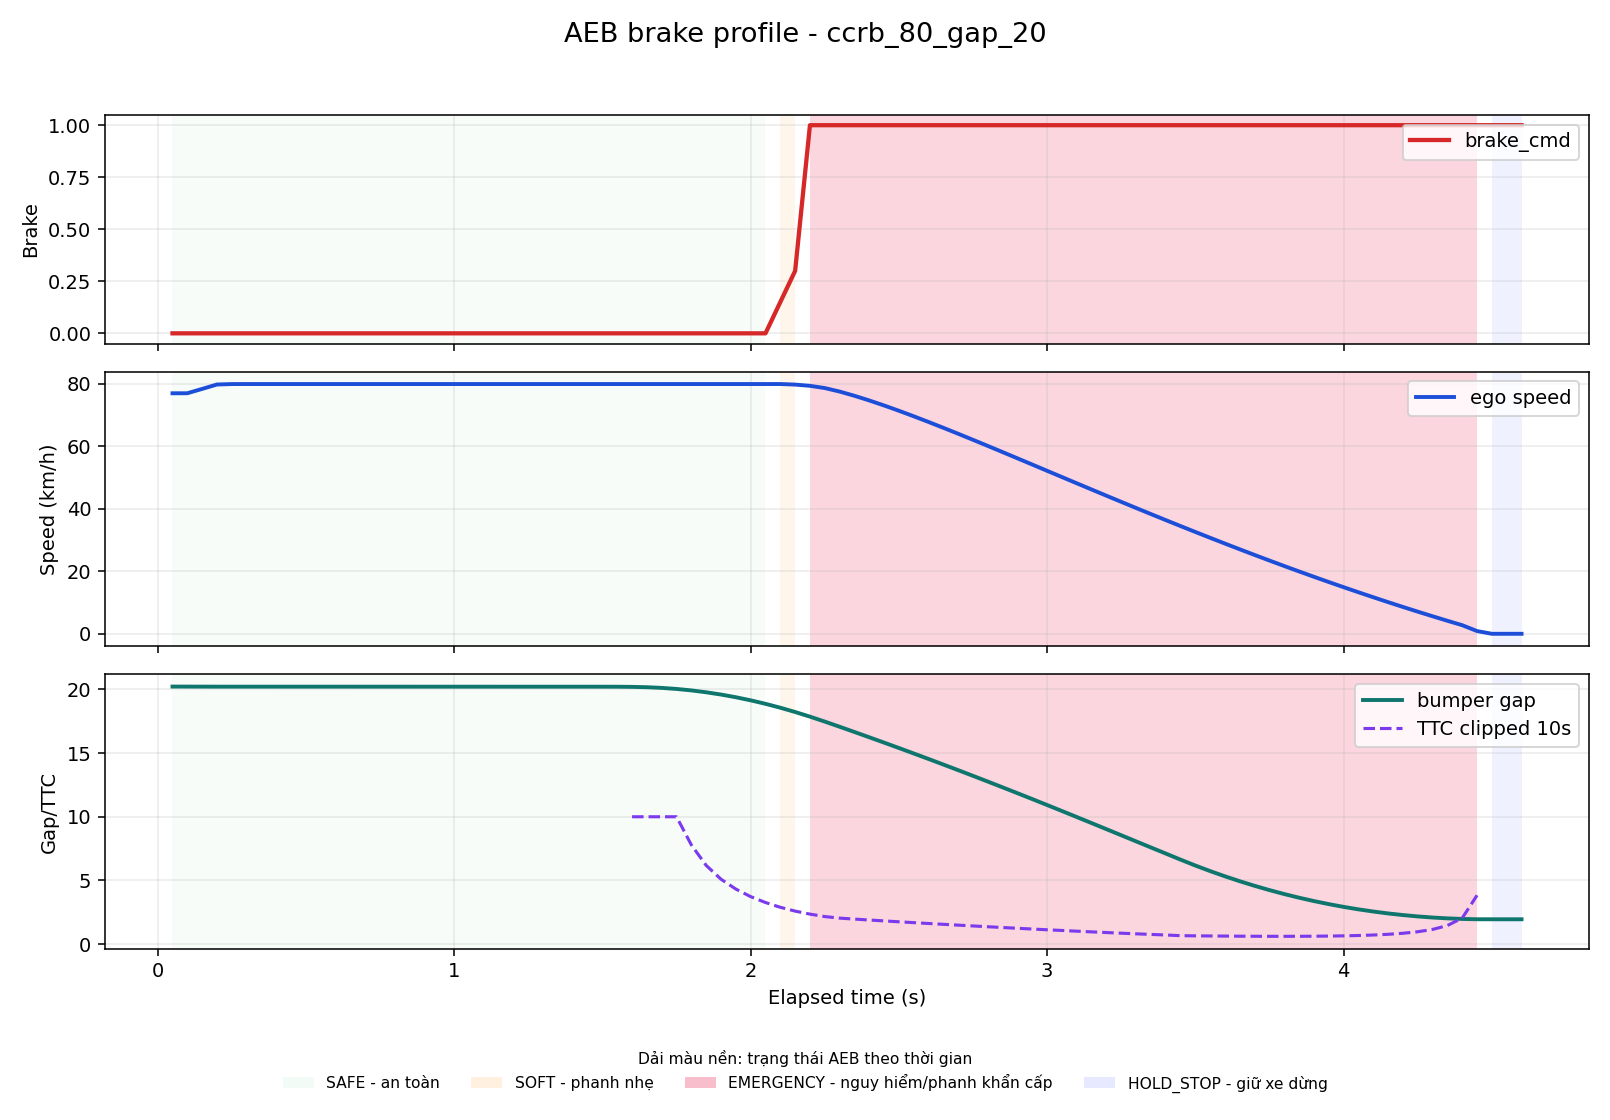
\includegraphics[width=0.49\columnwidth]{evidence/brake_profile_ccrb_80_gap_20.png}
  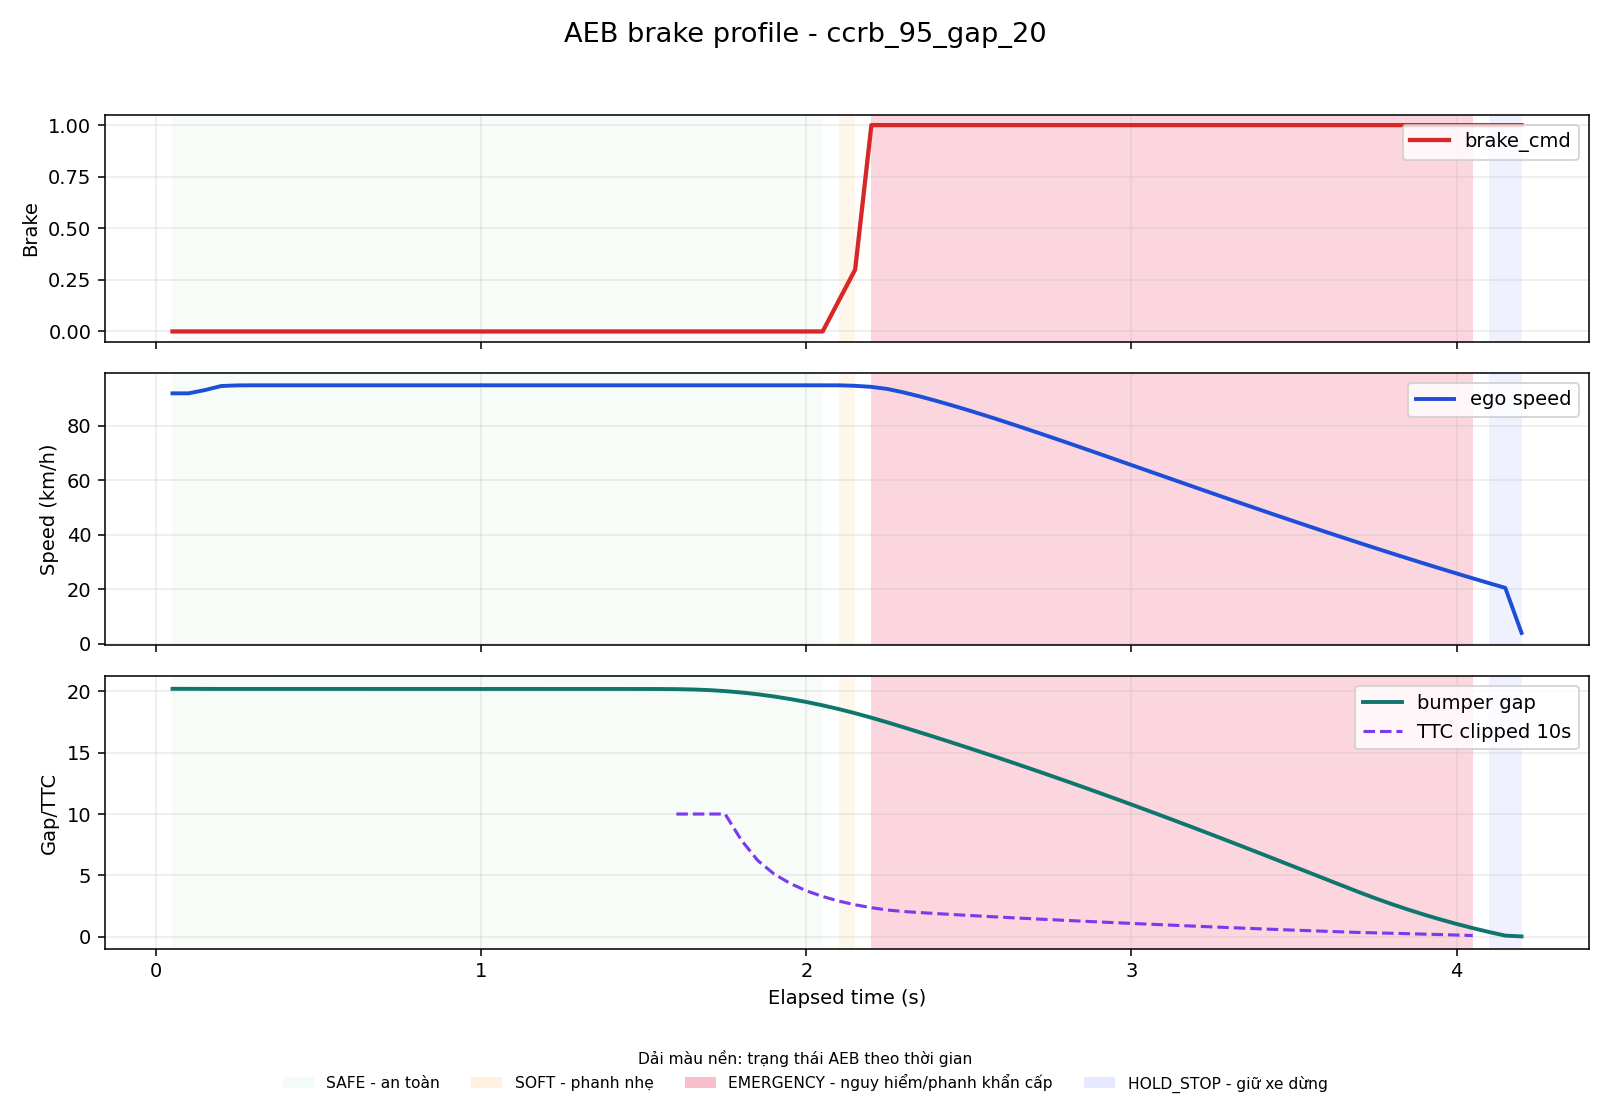
\includegraphics[width=0.49\columnwidth]{evidence/brake_profile_ccrb_95_gap_20.png}
  \caption{CCRb gap đầu 20~m: đạt tại 80~km/h (trái) và collision tại 95~km/h
  (phải).}
  \label{fig:ccrb}
\end{figure}

\subsection{Biên cut-in muộn}
Với cut-in, rủi ro chỉ có thể hành động sau khi target vào hành lang quỹ đạo và
nhận được xác nhận radar/camera dùng được. Case 80/50 phanh ở 10.46~m và đạt;
case 100/60 phanh ở 7.26~m rồi collision (Hình~\ref{fig:cutin}). Điều này cho
thấy trade-off chứ không chứng minh lợi ích thành phần: mở rộng corridor hoặc bỏ
camera permission có thể kích hoạt sớm hơn nhưng cũng có thể tăng phản ứng với
xe làn bên. Cần ablation radar-only/camera-gated đối xứng trước khi quy nguyên
nhân.

\begin{figure}[t]
  \centering
  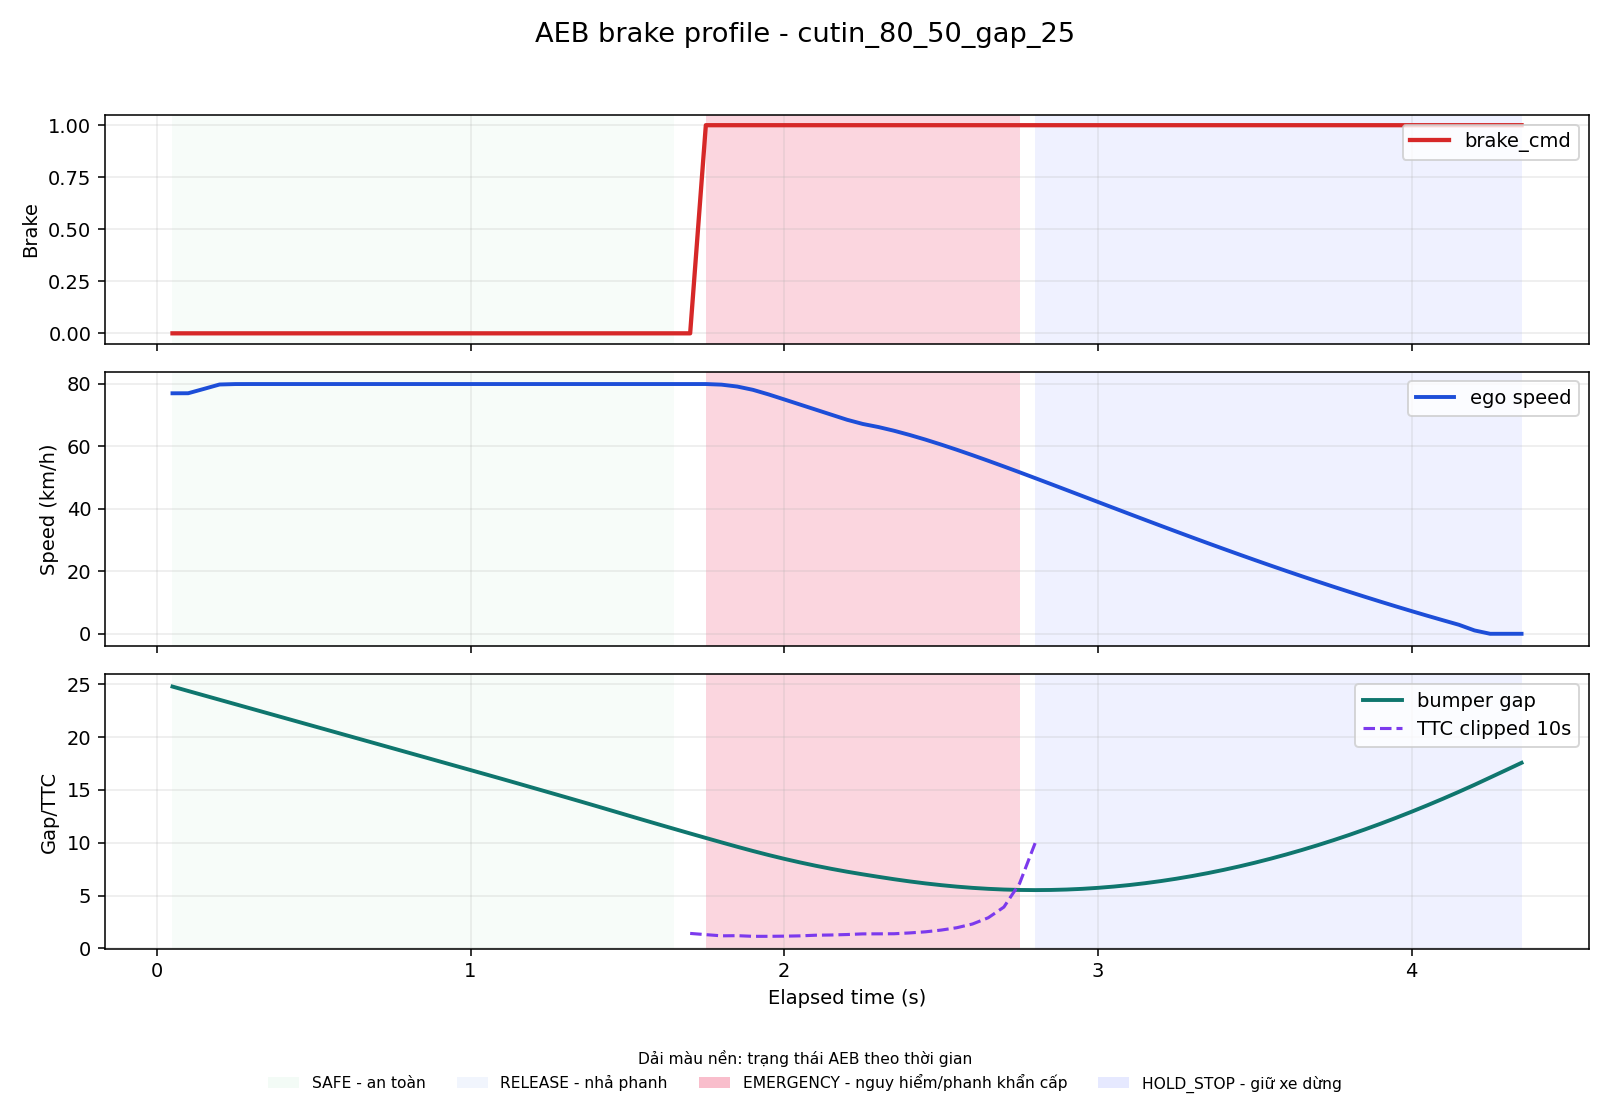
\includegraphics[width=0.49\columnwidth]{evidence/brake_profile_cutin_80_50_gap_25.png}
  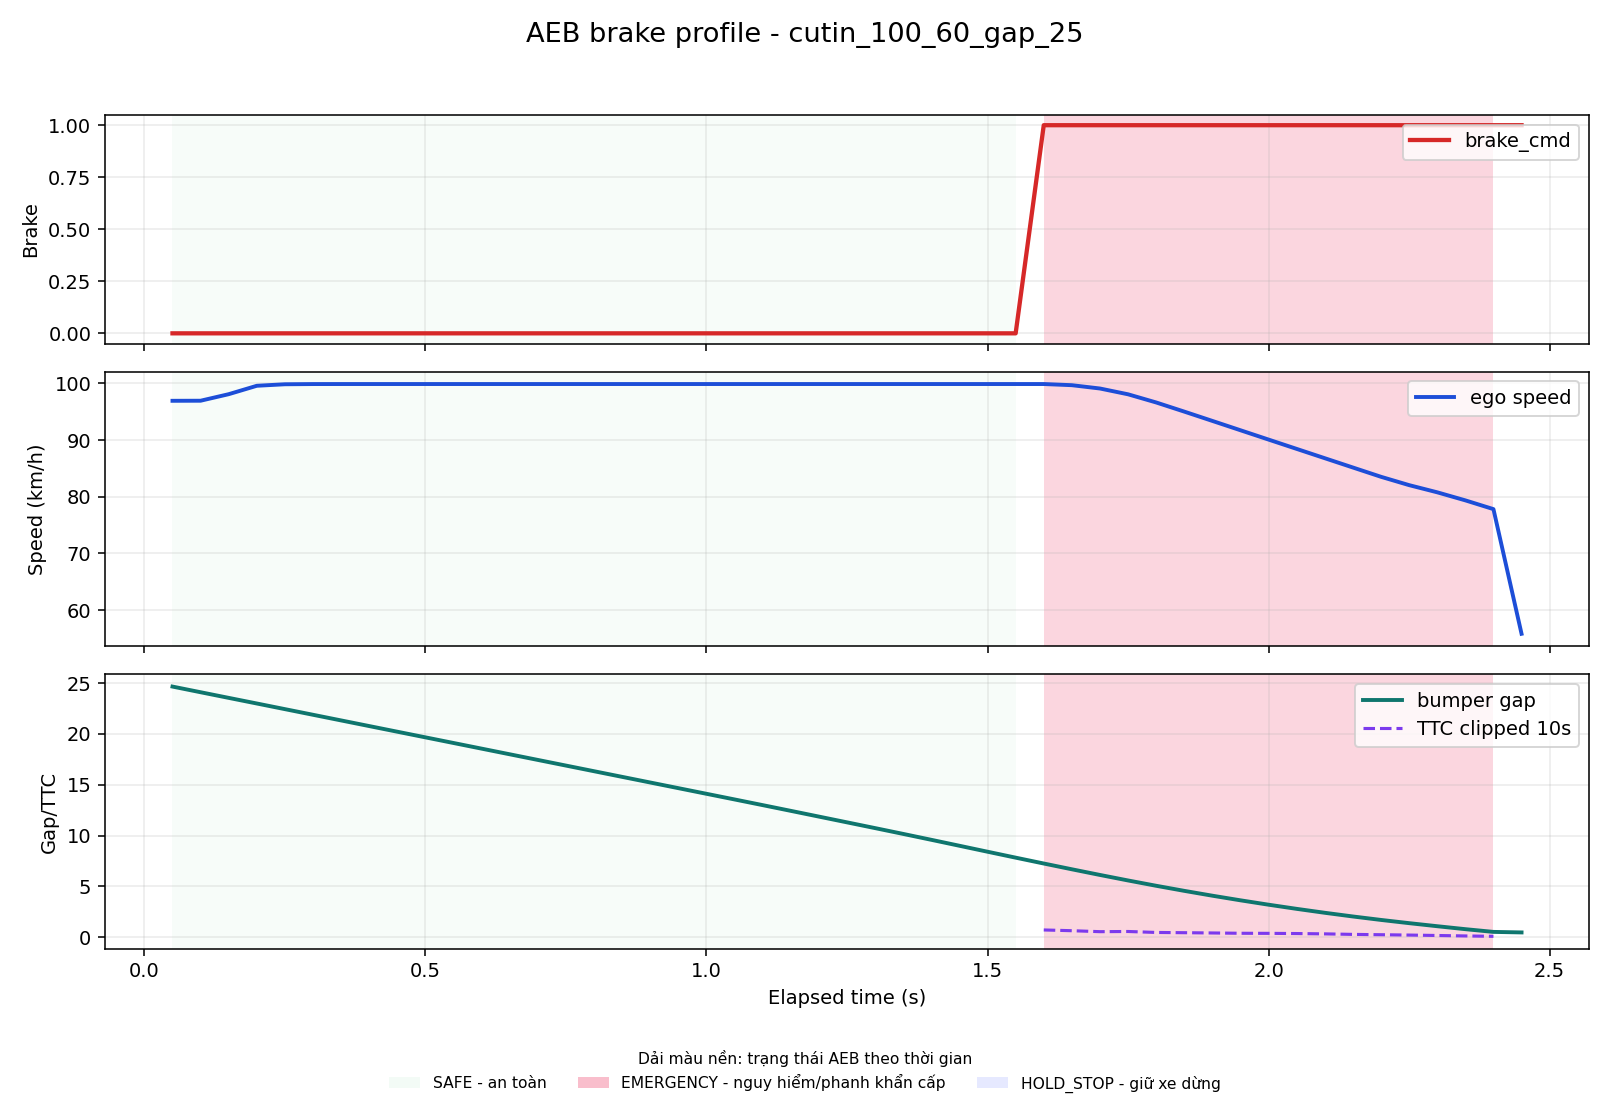
\includegraphics[width=0.49\columnwidth]{evidence/brake_profile_cutin_100_60_gap_25.png}
  \caption{Cut-in gap đầu 25~m: đạt tại 80/50~km/h (trái) và collision tại
  100/60~km/h (phải).}
  \label{fig:cutin}
\end{figure}

\subsection{Evidence chứng minh điều gì}
Ba kết luận có mức độ hỗ trợ khác nhau. Thứ nhất, hệ sensor-to-brake đầy đủ hoàn
thành mọi case mục tiêu trong một cấu hình CARLA cố định. Đây là existence result
end-to-end: điểm radar, detector, target gate, risk logic và chấp hành cùng tham
gia. Thứ hai, sweep tham số chỉ ra biên có cấu trúc trong tập run đã ghi: fail
CCRb cùng có gap ngắn nhất; fail cut-in kết hợp cặp tốc độ cao nhất với gap ngắn
nhất. Thứ ba, khoảng cách phanh đầu trong log cho thấy chuyển động target và thời
điểm vào quỹ đạo có ý nghĩa cùng tốc độ ego tuyệt đối.

Evidence không tách riêng module tạo ra kết quả. Không có ma trận run lần lượt bỏ
track confirmation, predicted path, camera permission, stopping margin hoặc
staged PID. Cũng không có baseline binary, radar-only hay perfect-perception trên
cùng 66 cấu hình. Vì vậy các câu như ``fusion tăng an toàn'', ``PID giảm jerk''
hay ``path gate giảm false brake'' sẽ vượt quá thí nghiệm. Kết quả bảo vệ được
là hành vi của cấu hình tích hợp.

\subsection{Liên hệ với hệ thống gần nhất}
So với bộ xác nhận do radar dẫn hướng trên xe thật của Akula \emph{và cs.}
\cite{akula2026radarguided}, nghiên cứu này có external validity yếu hơn và không
có lợi thế latency để claim. Camera ở đây nghiêm ngặt hơn về ngữ nghĩa--hỏi
mục tiêu có phải \emph{car}--nhưng phải trả chi phí model học và dữ liệu trong
domain. So với Zhang \emph{và cs.} \cite{zhang2023curved}, nghiên cứu mô tả cách
tạo target từ sensor thay vì bắt đầu bằng hazard đã nhận dạng, nhưng controller
không hiệu chuẩn với phần cứng. So với CARLA DVS \cite{feng2025dvs}, bài báo tập
trung động học do radar cung cấp thay vì tốc độ cập nhật ảnh. Khác biệt này định
vị baseline, không chứng minh hơn kém vì dataset, platform và tiêu chí khác nhau.

\subsection{Hàm ý kỹ thuật}
Các fail giữ lại gợi ý hai thí nghiệm tiếp theo. Với CCRb, cần lấy mẫu dày quanh
80--95~km/h và 20--30~m, đồng thời ghi target deceleration và brake onset so với
mốc 1.5~s. Với cut-in, cần factorial comparison thay đổi corridor width, số frame
xác nhận target và camera permission, đồng thời đo collision lẫn false brake trên
case xe làn bên đối xứng. Chỉ nên thêm lateral velocity hoặc time-to-lane-entry
nếu baseline chứng minh path-entry timing là giới hạn.

\section{Nguy cơ đối với tính hợp lệ}
\subsection{Internal và construct validity}
Ngưỡng rủi ro, cluster gate, temporal confirmation và PID gain được tune trong
cùng project trước final sweep. Không có protocol tối ưu scenario held-out được
ghi nhận, nên 38/38 có thể phản ánh một phần kiến thức về cấu hình. PASS cũng là
construct nhị phân: min gap 0.51~m đạt trong khi collision fail, nhưng không chấm
mức độ nghiêm trọng, comfort, tính phù hợp của can thiệp hay residual speed. Tập
cuối chỉ có hazard, nên đo missed/late intervention trực tiếp hơn unnecessary
intervention.

Mỗi cấu hình chỉ chạy một lần, không có seed ngẫu nhiên, confidence interval hay
ablation đối xứng. Vì vậy 63/66 là số case cấu hình, không phải reliability. Repo
check-in có evidence summary và plot nhưng thiếu CSV/JSON raw cuối được dẫn; các
giá trị aggregate và đại diện không thể tính lại độc lập chỉ từ checkout này.

Radar CARLA trả detection trừu tượng thay vì ADC, range--Doppler, CFAR, clutter
hay production tracking. Nhãn camera, calibration, map height và weather đều
thuộc domain simulator. Cửa sổ match 0.35~s dùng wall time thay vì simulation
time nên tải tính toán có thể đổi độ dài trong mô phỏng. Chưa đo phân bố latency
end-to-end. Test không xét lặp nhiều lần, thời tiết xấu, pedestrian, xe hai bánh,
ma sát lốp--đường, trễ thủy lực, ABS chi tiết hay phần cứng thật. Euro NCAP chỉ
truyền cảm hứng họ scenario \cite{euroncap_aeb}; ISO~15623 chỉ truyền cảm hứng
đại lượng cảnh báo va chạm \cite{iso15623}. Không tài liệu nào tạo chứng nhận.

\subsection{External và reproducibility validity}
Mọi ảnh detector và scenario cuối nằm trong domain simulator hẹp. mAP cao trong
domain vẫn có thể đi cùng association giòn ở map, hình dạng xe, che khuất, ánh
sáng hoặc calibration khác. Evidence pack ghi path tới CSV/JSON nhưng các file
này không có trong checkout. Report, plot, config và summary được check-in hỗ trợ
truy vết manuscript, nhưng chưa đủ rerun/tính lại độc lập nếu thiếu CARLA 0.9.11,
model artifact và log. Gói replication hoàn chỉnh cần pin CARLA image, môi
trường Python, model hash, random seed, source commit và toàn bộ summary sinh ra.

\section{Kết luận}
Bài báo mô tả baseline AEB sensor-to-brake trong CARLA: điểm radar thưa trở thành
object đã xác nhận và liên quan quỹ đạo; YOLO cấp quyền ngữ nghĩa tầng muộn; TTC,
biên dừng và staged PID khép kín vòng điều khiển. Cả 38 cấu hình dải mục tiêu đều
đạt, trong khi 3/28 cấu hình stress va chạm. Các fail xác định biên tốc độ cao--
gap ngắn và cut-in muộn thay vì bị loại khỏi kết quả. Bước tiếp theo có thể bảo
vệ được là ablation radar-only so với camera-gated lặp theo seed, đồng bộ theo
simulation time, phát hành raw artifact đầy đủ, rồi mới dùng model sensor và
actuator thực tế hơn trước mọi claim an toàn đường bộ.

\balance
\bibliographystyle{IEEEtran}
\bibliography{references}
\end{document}
